\section{Vertical Slice Demonstrator System}

\subsection{Overview and methodology}

\noindent The flexible architecture described above lends itself to an early technical demonstration of the system. The main goal of the demonstration system is to identify possible problems in the architecture design and, hopefully, find solutions. We would study, measure and optimize trigger latency and efficiencies at different stages of the system using hardware prototypes being developed. This will involve extensive simulation work, to guide the hardware implementation and to compare actual measurements with expectations. A possible Vertical Slice Demonstration System is shown in Figure~\ref{fig:VS_TBench}. Each stage is described in more detail in the following sections. For simplicity, we will often use the specific configuration with eight Data Input Boards and four Pattern Recognition Boards as an example. The architecture is flexible enough to allow for different configurations, so we plan to decide only at a later time which specific configuration we will actually use use for the demonstration system.

\begin{figure}[ht!]
\centering
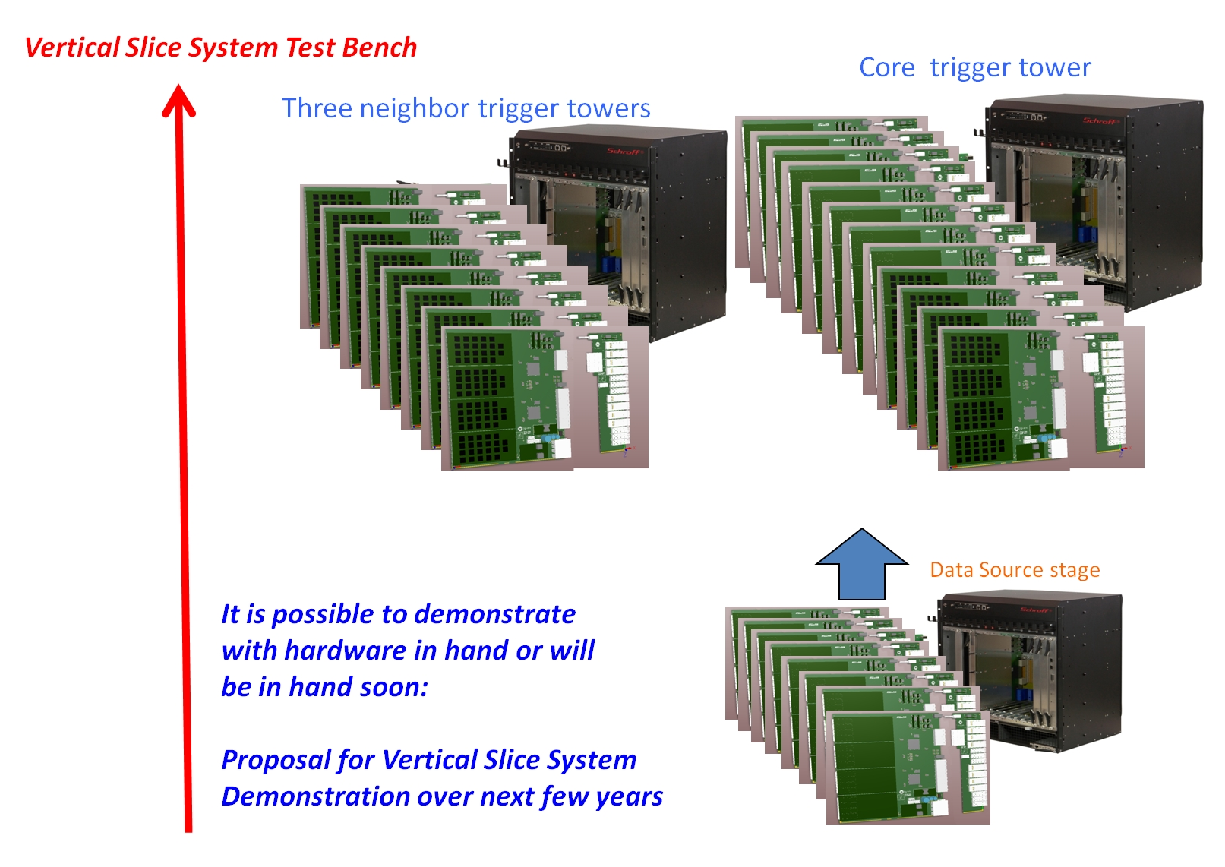
\includegraphics[width=0.7\columnwidth]{Plots/VSTBench.eps}
\caption{Vertical slice test bench principle.}
\label{fig:VS_TBench}
\end{figure}

\subsection{Data Source Stage}

\noindent The Data Source mimics the data flow out of the upgraded Phase II outer-tracker running at the HL-LHC. It will drive 300+ fibers (one/module) to the trigger tower under study exactly as the data were coming from the real detector at high luminosity and full speed. Each fiber connection will transmit data at 3.2Gbps payload, in the same way as the actual modules in the future real system. The data will be derived from simulation, appropriately coded, stored into on-board memories, and then played back at full speed.

\subsection{Data Input}

\noindent The Data Input Blade (DIB) is responsible for receiving data from the upstream detector electronics (or Data Source output) and transferring them to the PRBs. Up to about 40 fiber links will be received by each DIB. These input links may terminate on the RTM or mezzanine cards. Input fiber links are nominally 3.25Gb/s payload. The Data Input Board will perform zero suppression, pack the stubs into a new format and send them to the PRBs. Current estimates indicate that a rate of about 200 stubs per event per trigger tower, which yields a data rate of roughly 256Gb/s (200 stubs*32bits/25ns) entering each trigger tower on average.

\noindent As an example, in the configuration with eight DIBs and four PRBs, each DIB will be receiving an average of about 256/8 = 32 Gb/s of stub data (after zero suppression). Each of the eight DIBs in the shelf sends data to four PRBs in a round-robin, time multiplexed fashion. Since data is sent to four PRBs, these transfers can take place at a quarter of the input rate, or 32/4 = 8Gb/s.


\subsection{Pattern Recognition Board}

\noindent Using again the special configuration above (8 DIB + 4 PRB), each PRB will be receiving 64 Gb/s stub data on average. While receiving the data and sending them to the mezzanine cards, each PRB will exchange data with the corresponding PRB, processing the same time slice, in the neighboring tower for data sharing in the overlap regions. In this case, each PRB can use four 40Gb/s links (QSFP) for the connections in the eta and phi directions, and four 10Gb/s links (SFP+) can be used for data sharing in the "diagonal" directions (see Figure below for the shelf interconnections). The PRB FPGA drives data received from the DIBs to the Pattern Recognition Mezzanine (PRM) boards. This can also be done in a 4x time multiplexed fashion. The 4x time multiplexed transfers from the PRB FPGA to the PRM would require a bandwidth of about 16Gb/s this way. This also means that each PRM must contain all of the patterns for the trigger tower in this special configuration.
 
\begin{figure}[ht!]
\centering
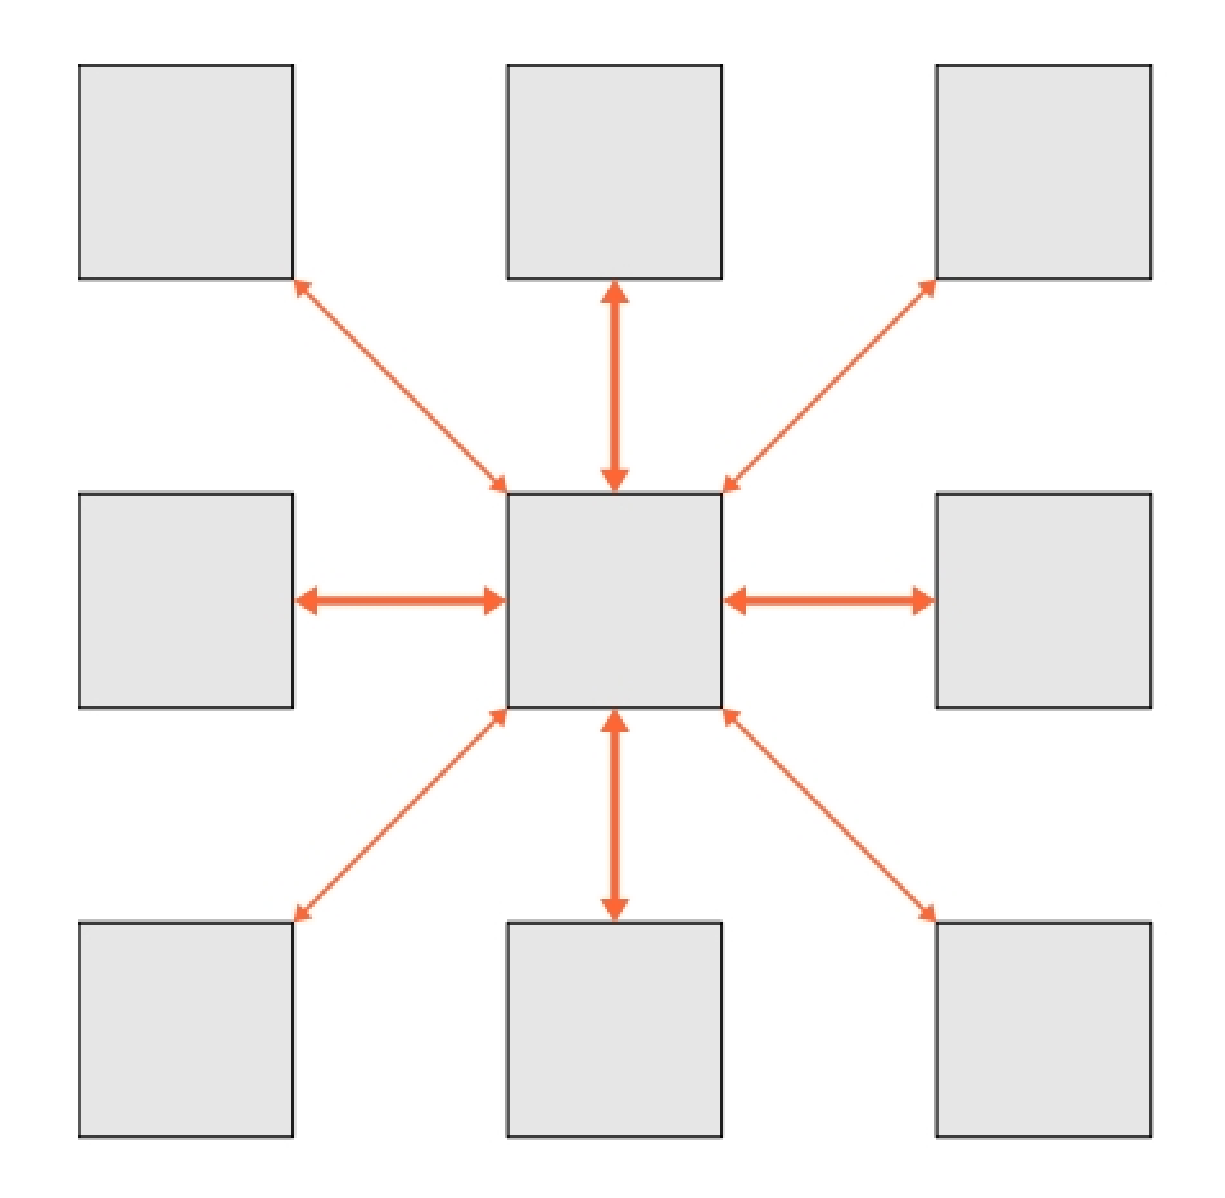
\includegraphics[width=0.4\columnwidth]{Plots/VSTBench_2.eps}
\caption{????}
\label{fig:VS_TBench_2}
\end{figure}


\subsection{Pattern Recognition Mezzanine Card}

\noindent Each PRB supports four Pattern Recognition Mezzanine (PRM) boards. These boards are based on the FMC standard and support high speed LVDS and SERDES connections to the PRB FPGA. Each PRM will contain an FPGA, on board memory to act as Data Buffer, and an array of pattern recognition associative memory (PRAM) devices.

\begin{figure}[ht!]
\centering
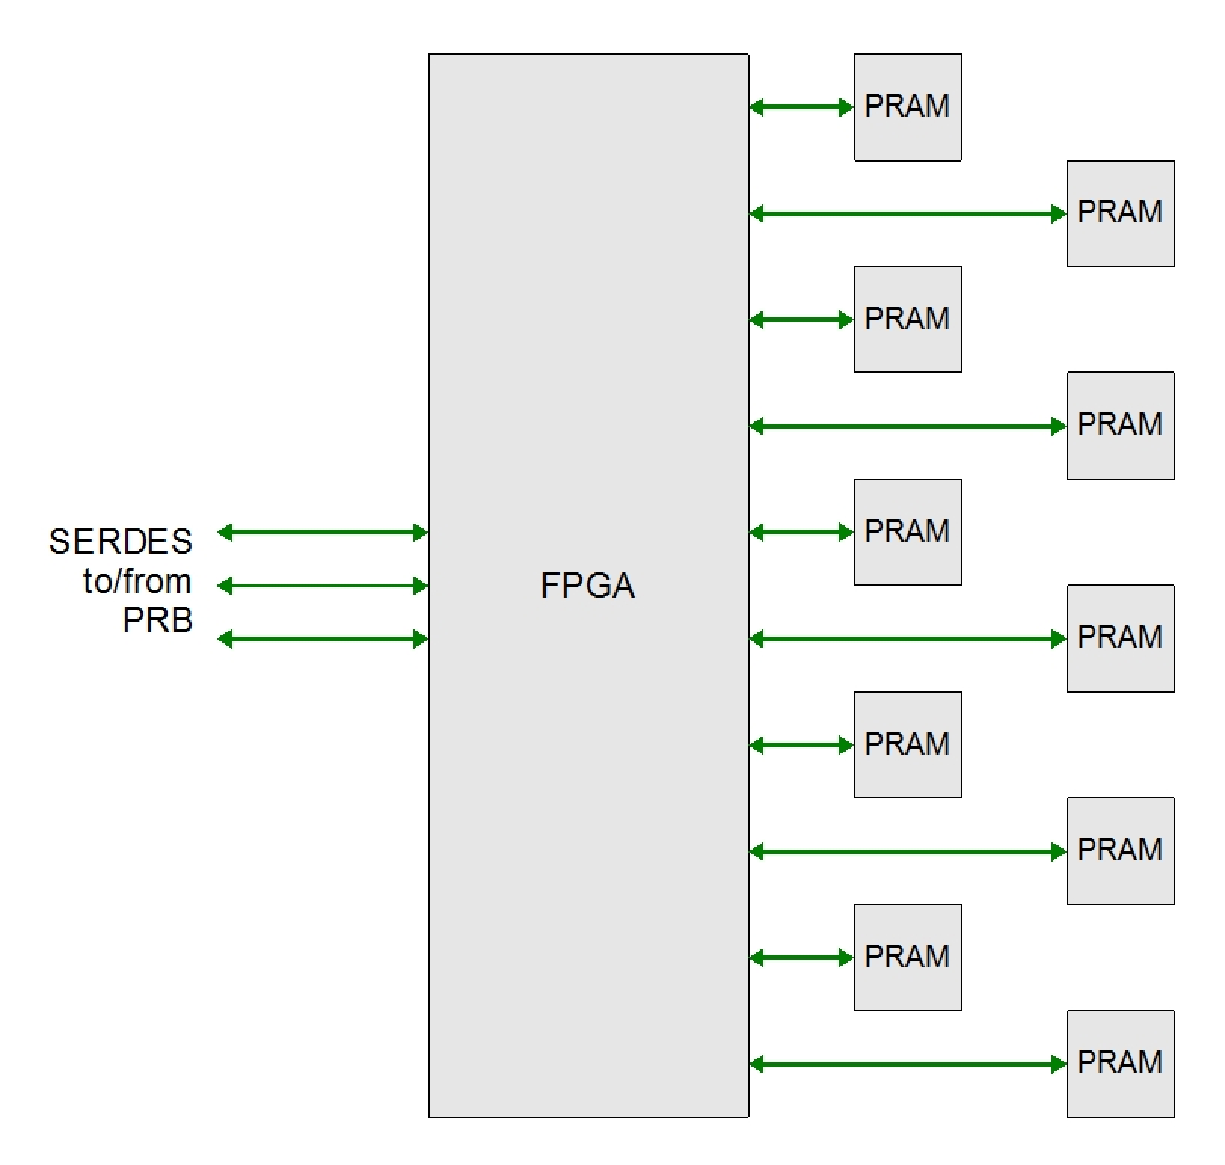
\includegraphics[width=0.6\columnwidth]{Plots/VSTBench_3.eps}
\caption{PRM working principle}
\label{fig:VS_TBench_3}
\end{figure}

\noindent In our example configuration, we need to support 16Gb/s between the PRB FPGA and the PRM.  This can be accomplished with an FPGA using three SERDES transceivers.  PRAM devices are attached to the FPGA using either a SERDES connection or multiple LVDS signal pairs.  The FPGA-PRAM channel bandwidth needs will be a fraction of the PRM input bandwidth, because only relevant stubs will be sent to the relevant AMchip covering the relevant regions of the trigger tower (see Figure~\ref{fig:VS_TBench_3}).

\noindent The PRM could be a logical successor to the test mezzanine card we have already designed. Future versions of the PRM will be designed to support different PRAM devices, such as AMCHIP0x (INFN) and the VPRAM0x (Fermilab). 

 
\subsection{PRAM and its Development}
  
\noindent As mentioned earlier, the CDF SVT-style Associative Memory chip (from now on we will call it PRAM, Pattern Recognition Associative Memory, to emphasis its purpose for HEP) is a departure beyond conventional CAMs. Like conventional CAMs, PRAMs store address patterns and look for matches between incoming hits and those addresses for a given detector layer. At this level, the match is expected to be either exact (Binary CAM) or partial (Ternary CAM) and an array of Match Flags is the typical output. A PRAM has an array of Match Flag Latches which capture and hold the results of the match until reset for the next event. As the hits from the various layers of the detector for the same event arrive, the PRAM is looking for more than simple matches from one candidate address to one or more stored address patterns. The PRAM organizes stored address patterns into roads, which are linked arrays of several stored address patterns from different detector layers. Each stored address pattern in a road is from a different layer in the detector system and these linked arrays represent a path or road that a particle might traverse through the layers of the detector (hence the name "road"). The ultimate goal of the PRAM is to match real particle trajectories to those roads. Like a conventional CAM, a PRAM flags a match when a candidate address matches a stored pattern address for a given detector layer. However, before the PRAM does anything with that match, it must find matches in all (or majority of) the elements (layers) that constitute a road.

\noindent It should be emphasized that compared to commercially available CAMs, such as Network Search Engine, the PRAM has the unique ability to search for correlations among input words received on different clock cycles. This is essential for tracking trigger applications since the input words are the detector hits arriving from different layers at different times. They arrive at the chip without any specific timing correlation. Each pattern has to store each fired layer until the pattern is matched or the event is fully processed. Even in the case of a level-1 trigger application, which is largely synchronous, this feature will still be important. One unique feature of this approach is that the pattern recognition of the event is done as soon as the last hit arrives, which makes the approach a promising candidate for L1 track trigger. However, the requirements for L1 track trigger application will be very different from that for L2, and the system interface of the chip has to be fully redesigned and the performance has to be optimized.

\noindent The PRAM pattern density can be improved by optimizing the design in single-layer chips (2D), using custom cell designs with smaller feature size technology. There is an R\&D effort by INFN using 65 nm technology to improve design for Atlas FTK application for L2 trigger (AMchip05 or 06). INFN has now in hands a 65 nm version prototype, developed for FTK purposes, which could be used for initial testing. INFN AM05 has been submitted recently, and the AM06 will be submitted in the Spring 2014. INFN AM06 for FTK with 128 Kpatterns is expected to become available in 2015.

\noindent  There is also an on-going R\&D effort at Fermilab using both conventional 2D and the emerging 3D technology to design future generation of PRAM chip~\cite{bib:VIP-11},\cite{bib:VIP-12} specifically for the needs of the L1 CMS tracking trigger needs (ProtoVIPRAM series). The first 2D prototype chip (ProtoVIPRAM01) is expected to arrive by the end of 2013.

\subsection{Track Fitting stage} 

\noindent The traditional CDF SVT/FTK-style track fitting stage can be used to benchmark the performance of this stage. We are exploring other new approaches as well, such as Hough transform algorithm and tracklet-based algorithm. All track fitting algorithms should be implemented in FPGA on the PRMs, therefore they can be studied and compared directly using the same vertical slice demonstration setup. More detailed description of the two new approaches will become available in this section later. As a reference, the traditional SVT/FTK-style track fitting is described below~\cite{bib:FTK-10}.

\noindent For a region of detector sufficiently small, a linear approximation gives helix parameters close to those of full helical fit. In other words, for a road narrow enough that a helical fit can be replaced by a simple linear calculation, each of the 5 helix parameters ($p_i$) can be calculated as the vector product of prestored constants ($a_{ij}$) and the hit coordinates ($x_j$): $p_i = a_{i0} + \sum_{i=1}^{N} a_{ij}x_{j}$  where N is the number of coordinates on the track, one for each SCT layer and two for each pixel layer.  Since there are more than 5 coordinates, there are additional linear equations that correspond to constraint equations, again where the constants are prestored.  There are (N - 5) such equations.  

\noindent This linear approximation gives near offline resolution for regions considerably wider than a single road.  A single set of constants will be used for each sector of the detector. The width of the sector at each silicon layer is the size of a physical detector module.  Per sector, 5�( N + 1) constants are needed for the helix parameters, and (N - 5)�( N + 1) constants are needed for the constraint equations.  The total number of fit constants (FC) per sector is thus N�(N + 1).

\noindent Will add some description here about CDF Gigafitter performance with FPGAs~\cite{bib:Ann-09}� etc. also with FTK most recent performance with modern FPGAs�

\subsection{Simulation efforts}

\noindent Simulation software plays an essential role in the development of a tracking trigger for CMS as it provides crucial input to the system design and hardware development. It is, therefore, imperative to have a robust and efficient simulation framework at the early stage of the project. The efforts to develop simulation software can be divided into the following tasks:

\begin{enumerate}
\item {\bf Data Format/Flow}: this part of the framework defines data formats and simulates the flow of the data at all stages from the tracker front-end electronics (transmitting hits associated with stubs) to the Layer-2 of the system (transmitting L1 tracks). This package should include detailed emulation of every stage of the data transmission including:
\begin{itemize}
\item Front End->Data Input Boards
\item Data Input Board-> Pattern Recognition Board
\item Pattern Recognition Board-> AM Mezzanine
\item Transmission of matched patterns from AMchip to the track fitting FPGA
\item Transmission of L1 tracks to downstream
\end{itemize}

\item {\bf AM simulation}: this part of the framework defines geometry of the trigger towers, this package is close connected to the previous and following packages and provides the expected output geometry used in the construction of the hits and further on the roads.

\item {\bf Pattern Bank Generation}: generates pattern bank, performs pattern matching and is interface-able with track fitting simulations. There is an existing framework in CMSSW, which serves this role and the Lyon group provides development and support for it. The main effort here should be aimed at improving the current performance of the package, namely addressing limitations related to speed and memory consumption.

\item {\bf Track Fitting}: this package is closely connected with the core AM simulations and provides functionality for emulating the FPGA-based track fitting stage. It should allow individual users to quickly access matched roads and associated hits, implement novel track fitting algorithms and test their performance.

\item {\bf Integration}: in order to have a complete bit-level emulator of the tracking trigger system, integration of the packages outlined above is necessary. The work here is to integrate, streamline and validate functionality of the full emulator.

\item {\bf GT interface}: this part of the framework provides simulation of the interface between the L1 tracks and the outputs of the calorimeter and muon triggers. This part should be developed in close collaboration with groups working on the upgraded calorimeter and muon L1 trigger systems

\item {\bf Fast simulation}: based on the SVT and FTK experience, it is reasonable to expect that the development of the full software suite outlined above will take a long time (years). On the other hand, improvements in the performance of CMS due to the availability of a tracking trigger need to be quantified on a much shorter time scale. It may, therefore, be advisable to invest in the development of a "light" tracking trigger simulation framework. The goal of this package would be to mimic the L1 tracking trigger performance by using offline hit/track collections and applying parametric efficiencies, fake rates and resolutions.

\item {\bf Vertical Slice Demonstration System Firmware and Software}: In addition to the emulators, a number of software and firmware packages will have to be delivered for each hardware component of the demonstrator. This includes hardware access software, low-level board validation software, integration software and monitoring software. The firmware for each component includes: core functionality firmware, validation firmware and algorithmic firmware.

\end{enumerate}

\clearpage
